\documentclass[../main/main.tex]{subfiles}

\newdate{date}{17}{03}{2020}

\begin{document}

\marginpar{ \textbf{Lecture 3.} \\  \displaydate{date}. \\ Compiled:  \today.}

To be more precise, in the previous derivation we have implicitely assumed that in all the cases the \( i \)  and \( j \)  coefficients where different. In order to be complete, we have also to take into account the \( i = j \) case; the result is the number operator \( \hat{n}_i = b_i^\dag b_i \).
Again, this is done explicitely for the kinetic energy term, but for the potential energy contribution the computation results more complicated.

Now, summurazing the contribution corresponding to the kinetic energy term and potential energy term we can rewrite the equation in the second quantization formalism
\begin{equation}
  i \hbar \pdv{}{t} \ket{\psi (t)} = \hat{H} \ket{\psi (t)}
  \label{eq:3_2}
\end{equation}
where \( \hat{H}  \) is an operator in the abstract occupation-number space, expressed in terms of \( b_i^\dag \) and \( b_i \):
\begin{equation}
  \hat{H} = \sum_{ij}^{} b_i^\dag \bra{i}T \ket{j} b_j +
  \frac{1}{2} \sum_{\substack{ij \\ kl} }^{} b_i^\dag b_j^\dag \bra{ij} V \ket{kl} b_l b_k
  \label{eq:3_3}
\end{equation}
\begin{remark}
  In the second quantization formalism the matrix elements \( \bra{i}T \ket{j}   \) and \( \bra{ij}V \ket{kl}   \) are simply complex numbers, while the quantum statistics is now incorporated into the \( b_i^\dag,b_i \) operators (with their commutation properties).
\end{remark}
Equation \eqref{eq:3_2} and \eqref{eq:3_3} toghether restate the Schr$\ddot{o}$dinger euqation in second quantization, and all of the statistics and operator properties are contined into creation and destruction operators. The physical problem is clearly unchanged by the new formulation. In particular the coefficients \( f \) specify the connection between first and second quantization.

For every solution \cite{fetter} to the original time-dependent many particle Schr$\ddot{o}$dingereuqation there exists a set of expansion coefficients \( f \). Given this set of expansion coefficients \( f \), it is possible to construct a solution to the problem in second quantization, as shown above. Conversely, if the problem is solved in second quantization, we can determine a set of expansion coefficients \( f \), which then yield a solution to the original time-dependent many particle Schr$\ddot{o}$dinger equation.

\begin{figure}[h!]
\begin{minipage}[c]{0.5\linewidth}
\centering
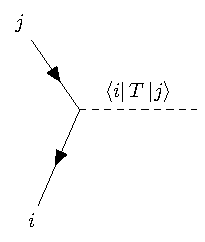
\includegraphics[width=0.7\textwidth]{../lessons/3_image/1.pdf}
\end{minipage}
\begin{minipage}[]{0.5\linewidth}
\centering
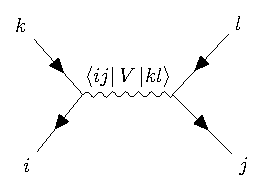
\includegraphics[width=0.8\textwidth]{../lessons/3_image/2.pdf}
\end{minipage}
\caption{\label{fig:} It is interesting to see a graphical representation of one and two-particle operators in the second quantization formalism. The incoming/outcoming arrows represent initial/final states. On the left, the dashed line represents the transition amplitude for one-particle process, while on the right, the sinusoidal lines represents the transition amplitude for two-particle process (for instance the Coulomb interaction). As we will see in the future, this representation is strictly connected to Feymann diagrams.}
\end{figure}

\subsection{Case: fermions particles}

Let us now repeat the same procedure for fermions particles and in particular let us decompose the \( N \)-body wave function as:
\begin{equation*}
  \psi (x_1,\dots,x_N,t) = \sum_{E_1,\dots,E_N}^{} c(E_1,\dots,E_N,t) \varphi _{E_1} (x_1) \dots \varphi _{E_N} (x_N)
\end{equation*}
The difference is that now the time dependent \( c \) coefficients are antisymmetric in order to respect the symmetry of the system:
\begin{equation*}
  c(\dots,E_1,\dots,E_j,\dots,t) = - c(\dots,E_j,\dots,E_i,\dots,t)
\end{equation*}

Hence we should have \( E_i \neq E_j \), otherwise we would obtain \( c=0 \). As a conseuqunce, we cannot have two particle in the same quantum state (\textbf{Pauli exclusion principle})\marginpar{Pauli exclusion principle} and the occupation number \( n_i \) for each state can assume only the value \( 0 \) or \( 1 \).
As done for the boson case, we can arrange the quantum numbers in the coefficient \( c \) in an increasing sequence as \( c(\dots,E_i^0< E_j^0<E_k^0, \dots,t) \) and introduce \( \bar{c}  \) coefficients:
\begin{equation*}
  \bar{c} (n_1,n_2, \dots, n_ \infty ,t)
\end{equation*}
Actually, the procedure is the same as for bosons: we want to expand the  \( N \)-body wave function. The difference is that for fermions the occupation number can be only 0 or 1, hence the \( \psi  \) can be written as:
\begin{equation*}
  \psi (x_1, \dots,x_N,t) = \sum_{n_1, \dots, n_ \infty = 0}^{1}
  f(n_1, \dots, n_ \infty ,t) \Phi _{n_1,\dots,n_ \infty } (x_1,\dots,x_N)
\end{equation*}
where now the \( \Phi  \) N-body time independent wave function should incorporate the symmetry of the system,
\begin{equation}
  \Phi _{n_1,\dots,n_ \infty } (x_1, \dots, x_N) = \sqrt{\frac{\prod_{i}^{} n_i!  }{N!}} \det\begin{bmatrix}
    \varphi _{E_1^0}(x_1)& \dots &\varphi _{E_1^0}(x_N) \\
    \vdots & & \\
    \varphi _{E_N^0}(x_1) & \dots & \varphi _{E_N^0}(x_N)
  \end{bmatrix}
\end{equation}
where we are considering the normalized determinant (\textbf{Slater determinant}). The first line in the matrix corresponds to the occupation of the first state by all the possible particle of the system and similarly for the other rows.

The \( \{ \Phi (\dots) \}   \) forms a complete set of orthonormal, antisymmetric, time-independent many-particle wave functions. Hence, by going from the coordinate space representation (\( \Phi _{n_1 \dots n_ \infty } (x_1, \dots, x_N) = \bra{x_1 \dots x_N} \ket{n_1 \dots n_ \infty }  \)) to the \emph{abstract} occupation number space we obtain:
\begin{equation*}
  \ket{\psi (t)} = \sum_{n_1, \dots, n_ \infty }^{} f(n_1, \dots, n_ \infty ,t) \ket{n_1, \dots, n_ \infty }
\end{equation*}
where there is the well known connection between the \( f \) coefficients and \( \bar{c}  \) coefficients:
\begin{equation*}
  f(n_1, \dots, n_ \infty ,t) = \sqrt{\frac{N!}{\prod_{i}^{} n_i!  }} \bar{c}  (n_1, \dots, n_ \infty ,t)
\end{equation*}
As for bosons, at this stage we should define suitable operators working in this abstract occupation-number space in such a way they incorporate the correct fermionic statistic\footnote{The \textbf{anticommutator} \( \{  \dots \}  \) is defined as  \( \{ A,B\} \equiv AB+BA   \) }:
\begin{equation}
  \begin{cases}
   \{a_i,a_j  \} = \{ a_i\dag,a_j\dag \} = 0 & \Rightarrow  \substack{   a_i a_j = - a_j a_i   \\   a_i^\dag a_j^\dag = - a_j^\dag a_i^\dag  }   \\
  \{ a_i, a_j^\dag \} = \delta _{ij}
  \end{cases}
\end{equation}
Let us check that these rules give the correct statistics (in particular, the occupation number cannot be larger than 1):
\begin{itemize}
\item Two particle cannot occupy the same state:
\begin{equation*}
  a_i^2 = \frac{1}{2} \{ a_i,a_i \} = {a_i^\dag}^2 = \frac{1}{2} = \{ a_i^\dag,a_j^\dag \}=0  \Rightarrow a_i^\dag a_i^\dag \ket{0} = 0
\end{equation*}
\item The occupation number operator is defined as \( \hat{n}_i=a_i^\dag a_i  \) and has the correct properties (for fermions), in fact:
\begin{equation*}
  \hat{n}_i^2 = a_i^\dag a_i a_i^\dag a_i = a_i^\dag (1 - a_i^\dag a_i) a_i = a_i^\dag a_i - \underbrace{{a_i^\dag}^2}_{=0}  \underbrace{a_i^2}_{=0}  = a_i^\dag a_i = \hat{n}_i
\end{equation*}
Hence, \( \hat{n}_i  \) is a \textbf{projector} which has the property that eigenvalues can be 0 or 1.
\end{itemize}
Moreover, remember that for bosons we have introduced also this additional relationship in Eq. \eqref{eq:2_10}. The same relations also hold for fermions \marginpar{Commutation properties}
\begin{subequations}
\begin{align}
   [a_i^\dag a_i, a_j^\dag] &= a_j^\dag \delta_{ij} \label{eq:3_1_1} \\
   [a_i^\dag a_i, a_j] &= - a_j \delta _{ij}
\end{align}
\end{subequations}
\begin{proof}[Proof of \eqref{eq:3_1_1}]
  Let us demonstrate explicitely only the first relation:
  \begin{equation*}
  \begin{split}
    [a_i^\dag a_i, a_j^\dag] &= a_i^\dag a_i a_j^\dag - a_j^\dag a_i^\dag a_i \\
    & = a_i^\dag a_i a_j ^\dag \qty(+ a_i^\dag a_j ^\dag a_i - a_i ^\dag a_ j ^\dag a_i) - a_j ^\dag a_i ^\dag a_i \\
    & = a_i ^\dag  \underbrace{\{ a_i,a_j ^\dag  \} }_{=\delta _{ij}}   - \underbrace{\{ a_i ^\dag , a_j ^\dag  \} a_i }_{=0} = a_j^\dag \delta _{ij}
  \end{split}
\end{equation*}
\end{proof}
Now, if we consider the commutator between the occupation number operators:
\begin{equation}
\begin{split}
[\hat{n}_i, \underbrace{ \hat{n}_j }_{a_j ^\dag  a_j} ]  &=  \hat{n}_i a_j ^\dag a_j - a_j ^\dag a_j \hat{n}_i   \\
& = \hat{n}_i a_j^\dag a_j \qty( - a_j ^\dag \hat{n}_i a_j + a_j ^\dag \hat{n}_i a_j  ) - a_j ^\dag a_j \hat{n}_i   \\
& = [\hat{n}_i, a_j ^\dag  ]a_j + a_j ^\dag [ \hat{n}_i , a_j ] )
= [a_i ^\dag a_i, a_j ^\dag ]a_j + a_j ^\dag [a_i ^\dag  a_i, a_j] \\
&= a_j ^\dag \delta _{ij} a_j + a_j ^\dag \qty(- a_j \delta _{ij}) = 0
\end{split}
\end{equation}
we can see that \( \hat{n}_i  \) and \( \hat{n}_j  \) commute: it allows the simultaneous diagonalization of the set \( \{ \hat{n}_i  \}   \), inline with the definition of the occupation number state vectors.

Giving these rules we can now write the generlalize abstract vector in this way: \marginpar{Generic state}
\begin{equation}
  \ket{n_1 n_2 \dots n_ \infty } = \qty(a_1^\dag)^{n_1}\qty(a_2^\dag)^{n_2} \dots \qty(a_ \infty ^\dag)^{n_ \infty } \ket{0}
\end{equation}
recalling that \( \qty(a_i^\dag)^{n_i} = 0 \, \forall n_i>1\) because of the exclusion principle.
In particular:
\begin{subequations}
\begin{align*}
   a^\dag \ket{0} &= \ket{1} \quad a^\dag \ket{1} = 0 \\
   a \ket{0} &= 0   \quad \quad \, a \ket{1} = \ket{0}
\end{align*}
\end{subequations}

Due to the anticommutator rules (\( a_j ^\dag a_k ^\dag = - a_k ^\dag a_j ^\dag  \)) it is essential to keep track of signs, for instance consider the  action of \( a_j^\dag \) into the state: \marginpar{Phase factor \( S_j \)}
\begin{equation*}
\begin{split}
  a_j^\dag \ket{n_1, n_2, \dots, n_ \infty }  &= a_j ^\dag \qty(a_1 ^\dag )^{n_1} \qty(a_2 ^\dag )^{n_2}  \dots \qty(a_ \infty  ^\dag )^{n_ \infty }  \ket{0}  \\
  & \overset{\text{if} j \neq 1}{=}  \qty(a_1 ^\dag )^{n_1} a_j ^\dag \qty(-1)^{n_1} \qty(a_2 ^\dag )^{n_2}   \dots \ket{0} \\
  & \overset{\text{if} j \neq 2}{=} \qty(a_1 ^\dag )^{n_1} \qty(a_2 ^\dag )^{n_2}  a_j ^\dag \qty(-1)^{n_1} \qty(-1)^{n_2} \dots \ket{0} \\
  & = \dots \dots
\end{split}
\end{equation*}
At the end one gets to \( \qty(a_j ^\dag )^{n_j}  \):
\begin{equation*}
  a_j^\dag \ket{n_1, n_2, \dots, n_ \infty }  = \underbrace{(-1)^{n_1+n_2+ \dots + n_{j-1}}}_{\equiv \text{phase factor} S_j}  \ket{n_1, \dots(n_j+1) \dots n_ \infty }
\end{equation*}
that is a state where we have and additional particle if the \( j \) state was empty (\( n_j=0 \)), otherwise, if the state was already occupied (\( n_j=1 \)), we get 0. The difference with the boson case is that now we have to take into account the \textbf{phase factor} \( S_j \).
Similarly if we apply the destruction operator:
\begin{equation*}
  a_j \ket{n_1, n_2, \dots, n_ \infty }  = S_j \ket{n_1, \dots(n_j+1) \dots n_ \infty }
\end{equation*}
Moreover, by combining the action of the two operators we have no phase factor:
\begin{equation*}
  a_j ^\dag a_j \ket{\dots n_j \dots} = n_j \ket{\dots n_j \dots}
\end{equation*}
Hence, we have seen efinition and properties for creation and destruction operators for fermions; now  we can repeat the same derivation as for bosons starting from the Schr$\ddot{o}$dinger equation:
\begin{equation*}
  i \hbar \pdv{}{t} \ket{\psi (t)} = \hat{H} \ket{\psi (t)}
\end{equation*}
We introduce the \( c \) coefficients and we write the corresponding equation for them, by focusing on the kinetic term:
\begin{equation}
i \hbar \pdv{}{t} c(E_1, \dots, E_N, t) = \sum_{k=1}^{N}  \sum_{E_k'}^{} c(E_1, \dots, E_k', \dots, E_N,t) \bra{E_k} T \ket{E_k'}
\end{equation}
the procedure is similar, but with the crucial difference that by reordering the quantum numbers on both sides of the equation one must carefully keep track of phase factors, since we are dealing with fermions.

At the end of the derivation \cite{fetter}:
\begin{equation*}
  (-1)^{S_j-S_i} \ket{\dots (n_i' +1) \dots (n_j'-1) \dots } = a_i ^\dag  a_j \ket{n_1' \dots n_ \infty '}
\end{equation*}
We obtain an expression for \( H \) in SQ which is formally equal (the quantum statistic difference is incorporated in the properties of the \( a_i, a_i ^\dag  \) operators!) to that for bosons:
\begin{equation}
  \hat{H} = \sum_{ij}^{} a_i^\dag \bra{i}T \ket{j} a_j +
  \frac{1}{2} \sum_{\substack{ij \\ kl} }^{} a_i^\dag a_j^\dag \bra{ij} V \ket{kl} \mathcolorbox{green!20}{a_l a_k}
\end{equation}
where the ordering of the final two operators in green is crucial (for bosons was irrelevant because the operators commute) to get that \( \hat{H}  \) is \emph{hermitian} and correct (if the order is inverted a minues sign appears in the potential energy term!).

\begin{remark}
The formal expression for the kinetic energy term:
\begin{equation*}
  \hat{T} \equiv \sum_{ij}^{} a_i ^\dag  \bra{i}  T \ket{j} a_j
\end{equation*}
can be generalized for any single-particle operator; for example to the total moment can be expressed as
\begin{equation*}
  \hat{\va{p}} = \sum_{ij}^{} a_i ^\dag  \bra{i} \va{p } \ket{j} a_j
\end{equation*}
\end{remark}


\section{Field operators}
Now, we make a step further considering but we still consider the second quantization formalism. Let us define \textbf{field operators} formed by the linear combination of creation and destruction operators: they create and destroy particles in a \emph{selected} point \( \va{x} \): \marginpar{Creation and destruction field operators}
\begin{equation}
  \begin{cases}
   \hat{\psi }_ \alpha  (\va{x}) \equiv  \sum_{\va{k}}^{} \varphi _{\va{k}, \alpha } (\va{x}) a_{\va{k}, \alpha }  \\
\hat{\psi }_ \alpha ^\dag   (\va{x}) \equiv  \sum_{\va{k}}^{} \varphi _{\va{k}, \alpha } ^\dag  (\va{x}) a_{\va{k}, \alpha } ^\dag
  \end{cases}
\end{equation}
where in the specific case of fermions we have the wave vector index \( \va{k} \) and the spin index  \( \alpha  \). We can see that by considering a linear combination of the creation and destruction operators with coefficients \(\varphi _{\va{k}, \alpha }   \), that are single-particle wave functions, we obtain new operators which depend on the spatial space coordinates.
Moreover, the \( \sum_{k}^{}   \) in the creation field operator can be interpreted as the sum of all possible ways to add a particle at position \( \va{x} \) through any of the basis states \( \varphi _{\va{k}, \alpha } \).

Crearly, for a \emph{homogeneous} system of electrons we can consider the single-particle wave function made by normalized plane wave
\begin{equation*}
  \varphi _{\va{k}, \alpha } (\va{x}) = \frac{e^{i \va{k} \vdot \va{x}} }{\sqrt{V} } \eta _{\alpha }
\end{equation*}
 where \( V \) is the volume and \( \eta_ \alpha   \) the spin function which can be \( (1 \,\, 0 )^T\) or \( (0\,\, 1 )^T\).

For example, we want to write the kinetic term in second quantization using these new fields: \marginpar{Kinetic term with field operators}
\begin{equation*}
\begin{split}
  \sum_{ij}^{} a_i ^\dag \bra{i} T \ket{j} a_j & \underset{\substack{i \rightarrow \va{k}, \alpha  \\ j \rightarrow \va{k}, \beta } }{\longrightarrow}  \sum_{\substack{\va{k} \alpha  \\ \va{k} \beta } }^{} a_{\va{k} \alpha } ^\dag \qty(\int_{}^{} \dd[3]{x} \varphi _{\va{k} \alpha } ^\dag (\va{x}) \qty(- \frac{\hbar ^2 \grad _x^2}{2m}) \varphi _{\va{k} \beta } (\va{x}) )    a_{\va{k}, \beta } \sigma _{\alpha \beta } \\
  & = \sum_{\alpha \beta }^{} \delta _{ \alpha  \beta } \int_{}^{} \dd[3]{x} \underbrace{\qty(\sum_{\va{k} \alpha }^{} \varphi _{\va{k} \alpha } ^\dag (\va{x}) a_{\va{k} \alpha }^\dag  )    }_{\hat{\psi }_ \alpha ^\dag (\va{x}) } \qty(- \frac{\hbar ^2 \grad _x^2}{2m})
  \underbrace{\qty(\sum_{\va{k} \beta }^{} \varphi _{\va{k} \beta } ^\dag (\va{x}) a_{\va{k} \beta }^\dag  )    }_{\hat{\psi }_ \beta  (\va{x}) } \\
  & = \int_{}^{} \dd[3]{x} \sum_{\alpha \beta }^{} \hat{\psi }_ \alpha  ^\dag (\va{x})   \underbrace{\qty(- \frac{\hbar ^2 \grad _x^2}{2m}) }_{T (\va{x})} \hat{\psi _ \beta } (\va{x}) \delta _{\alpha \beta }
\end{split}
\end{equation*}
where in the first step we have explicitely expressed the matrix element, where the kinetic energy term is diagonal on the spin index. Then we have grouped these terms and we have seen that the combinations obtained correspond to the field creation and destruction operators. Finally we have written the expression in function of these fields.

It is easy to demonstrate that these new field operators, since are nothing else of linear combination of the previous defined creation and destruction operators, satisfy the same commutation or anticommutation relations. For instance for fermions
\begin{equation*}
\begin{split}
\{ \hat{\psi }_ \alpha (\va{x}), \hat{\psi }_ \beta ^\dag (\va{x}')   \}    &=  \sum_{\va{k} \va{k}'}^{}  \psi _{\va{k}, \alpha } (\va{x}) \psi _{\va{k}', \beta }^\dag (\va{x}')  \underbrace{\{ a_{\va{k}, \alpha }, a_{\va{k}', \beta } ^\dag  \} }_{ \delta _{\va{k},\va{k}'} \delta _{\alpha \beta }}  = \sum_{\va{k}}^{} \psi _{\va{k}, \alpha }(\va{x}) \psi _{\va{k}, \beta } ^\dag \delta _{\alpha \beta }  \\
& = \sum_{\va{k}}^{} \bra{\va{x}}  \underset{\text{completness}}{\ket{\psi _{\va{k}, \alpha }} \bra{\psi _{\va{k},\beta }}}  \ket{\va{x}'}  \delta _{\alpha \beta }
= \delta (\va{x}-\va{x}') \delta _{\alpha \beta }
\end{split}
\end{equation*}

\begin{table}[h!]
  \centering
\begin{tabular}{lll}
  \toprule
  \textbf{Bosons}  & \textbf{Fermions} & \textbf{Field Operators} \\
  \toprule
  \textbf{Commutation rules} & & \\
  \midrule
   \( [b_k,b_{k'}^\dag ] = \delta _{k,k'} \) & \( \{a_r,a_{s}^\dag \} = \delta _{r,s} \)&  \( [\hat{\psi }_ \alpha (x), \hat{\psi }_ \beta ^\dag (x')  ]_\pm = \delta _{\alpha \beta } \delta (x-x') \) \\
   \( [b_k,b_{k'}] = 0 \) & \( \{ a_r,a_s \}=0   \)& \( [\hat{\psi }_ \alpha (x), \hat{\psi }_ \beta (x')  ]_\pm = 0 \)\\
   \( [b_k ^\dag , b_{k'} ^\dag ] = 0 \) & \( \{ a_r ^\dag , a_s ^\dag  \} =0  \) & \( [\hat{\psi }_ \alpha ^\dag (x), \hat{\psi }_ \beta ^\dag (x')  ]_\pm = 0 \) \\
   \midrule
   \textbf{Important relations} & & \\
   \midrule
   \( [b ^\dag b, b] = - b \delta _{kk'} \) & \( [a_r ^\dag  a_r, a_s ^\dag ] = a_s ^\dag \delta _{rs} \)& \\
   \( [b ^\dag b , b ^\dag ] = b ^\dag \delta _{k k'} \) & \( [a_r ^\dag  a_r, a_s] = - a_s \delta _{rs} \)& \\
   \bottomrule
\end{tabular}
\caption{Commutation rules for creation and distruction operators, where the upper \( + \) sign refers to bosons, while the lower  \( - \) sign to fermions (respectively commutator or anticommutator).}
\end{table}



Also the interaction potential energy term can be expressed in terms of the field operators, so that we can rewrite in SQ the Hamiltonian with the field operators:
\begin{equation}
  \hat{H} = \sum_{\alpha }^{} \int_{}^{} \dd[3]{x} \hat{\psi }_ \alpha ^\dag  (\va{x}) T (\va{x}) \hat{\psi }_ \alpha (\va{x})
  + \frac{1}{2} \sum_{\alpha \beta }^{} \int_{}^{} \dd[3]{x}
  \int_{}^{} \dd[3]{x'} \hat{\psi }_ \alpha ^\dag (\va{x})
  \hat{\psi }_ \beta ^\dag (\va{x}') V (\va{x},\va{x}') \mathcolorbox{green!20}{\hat{\psi }_ \beta (\va{x}') \hat{\psi }_ \alpha (\va{x})          }
\end{equation}
where the order of the two final field operators, in green, should be at it is here due to the requirement that the hamiltonian is hermitian and that the fermionic statistic is correct.
The quantities \( \hat{\psi }  \) and \( \hat{\psi } ^\dag   \) are not wave functions, however, but field operators; thus in second quantization the fields are the operators and the potential and kinetic energy are just complex coefficients.






To summarize:
\begin{itemize}
\item in first quantization:
\begin{equation*}
  \int_{}^{} \dd[3]{x} \underbrace{\psi ^\dag (\va{x}) V (\va{x}) \psi (\va{x})}_{\bra{\psi } V \ket{\psi } }
\end{equation*}
where the \( \psi  \) are wave functions.
\item in second quantization:
\begin{equation*}
  \int_{}^{} \dd[3]{x} \hat{\psi }^\dag (\va{x}) V (x) \hat{\psi }(\va{x})
\end{equation*}
where the \( \hat{\psi }  \) are field operators and \( V(x) \) in the middle is just a complex coefficient.
\end{itemize}
Hence, the expressions for the potential term are very similar in both first and second quantization, but there is an important difference: in the second quantization the wave function are replaced with the fields.
Namely, the wave functions are "transformed" into (field) operators.

It is easy to extend the derivation to any other operator; for instance for a general, one-body operator.
\begin{example}{Quantum angular momentum}{}
For example in first quantization we have this term (quantum angular momentum, but could be any one body operator):
 \begin{equation*}
   J = \sum_{i=1}^{N} J (\va{x}_i)
 \end{equation*}
 where the \( i \) is a particle index. In second quantization, we can write this expression in terms of the coefficients:
 \begin{equation*}
   \hat{J} = \sum_{ij}^{} \bra{i} J \ket{j} c_i ^\dag c_j = \int_{}^{} \dd[3]{x} \hat{\psi } (\va{x}) J (x) \hat{\psi } (\va{x})
 \end{equation*}
 where now \( ij \) represents state index.
 We pointed out that in first quantization we have a sum over particles, while here we have sum over states: we used the same letters but the meaning is completely different!
\end{example}

\marginpar{Number density operator}
\begin{example}{Number density operator}{}
A useful quantity is the \textbf{number density operator}, which in first quantization can be written as
\begin{equation*}
  n (\va{x}) = \sum_{i=1}^{N} \delta (\va{x}- \va{x}_i)
\end{equation*}
Now, it is an easy exercise to demonstrate that in second quantization the expression is like
\begin{equation*}
  \hat{n} (\va{x}) = \sum_{ij}^{} \phi _{E_i} ^\dag  (\va{x}) \phi _{E_i} \va{x} c_i ^\dag c_j =
  \int_{}^{} \dd[3]{x} \hat{\psi } ^\dag (\va{x}') \delta (\va{x}- \va{x}') \hat{\psi } (\va{x}') = \hat{\psi }^\dag (\va{x}) \hat{\psi } (\va{x}')
\end{equation*}

The expression \( \hat{n} (\va{x}) =  \hat{\psi }^\dag (\va{x}) \hat{\psi } (\va{x}')    \)  in second quantization is formally similar to the familiar expresssion of quantum mechanics (in first quantization):
\begin{equation*}
  n (\va{x}) = \psi ^* (\va{x}) \psi (\va{x}) = \abs{\psi (\va{x})} ^2
\end{equation*}
that the probability density is given by the product of complex conjiugate wave function for the wave function itself, which corresponds to the square modulus of the wave function.
However, the meaning is different because in the first we have fields, while in the second we have wave functions.
\end{example}

\marginpar{Total-number operator}
\begin{example}{Total-number operator}{}
Similarly, the \textbf{total-number operator} in second quantization is:
\begin{equation*}
  \hat{N} = \int_{}^{} \dd[3]{x} n(\va{x})
  = \sum_{i}^{} c_i ^\dag c_i = \sum_{i}^{} \hat{n}_i =
  \int_{}^{} \dd[3]{x} \hat{\psi }^\dag (\va{x}) \hat{\psi }(\va{x})
\end{equation*}
this can be easily obtained just considering that the single-particle wave functions (in the field definition oeprators) are orthonormal.
\end{example}

It is easy to show that the commutator between the total-number operator and the Hamiltonian is zero:
\begin{equation}
  [\hat{N}, \hat{H}  ] = 0
\end{equation}
hence \( \hat{N}  \) can be diagonalized simultaneously with \( \hat{H}  \) (\( N= \)constant).

In conclusion, the second quantization formalism is just an alternative way to reformulate the original Schr$\ddot{o}$dinger equation. Now the idea is trying to apply it to our \( N \)-body problem.









\section{Application: Jellium model}
Now we try to apply the second quantization formalism to an interesting physical model: “\textbf{degenerate electron gas}” or \textbf{Jellium model}.
In particular, \emph{ “degenerate matter” means we are considering matter with high density, so high that the dominant contribution to its pressure rised from the Pauli exclusion principle}: we cannot force two electrons to occupy the same quantum state.

Many systems in the universe obey this property. For instance:
\begin{itemize}
\item electron gas in ordinary metals (Drude-Sommerfiled theory of metals);
\item plasma;
\item white dwarf stars. Ordinary stars cannot collapse due to the gravitational forcee bacause of the standard idrostatic pressure. In the interior of these particular dwarf stars, we have we have both \( \alpha  \) particles (He nuclei) and free electrons at high density, and the stability of the star is supported by the degeneracy pressure due to the Pauli exlusion principle. Hence, they not collapse because we cannot compress too much the electrons system if it is at high density.
\item Neutron stars: the principle is as the one for dwarf stars, but in this case the degenerate particles are not electrons but neutrons.
\end{itemize}

\marginpar{
    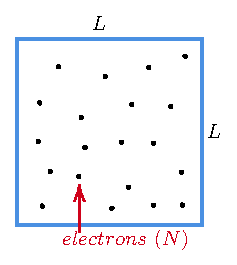
\includegraphics[width=\marginparwidth]{../lessons/3_image/3.pdf}
  \captionof{figure}{\label{fig:} Cubic box of side \( L \) with \( N \) electrons and uniform positive background.}
    }

We assume that the Jellium model is included in a cubic box of side \( L \), that is large. More specifically, we will assume that \( L \rightarrow \infty  \), in a way to focus only on bulk properties and to not deal with surfaces. In this box wa have essentially:
\begin{enumerate}
\item An interacting electron gas: \( N \) interacting electrons.
\item An uniformly distributed \emph{positive} background, to ensure that the total system is neutral.
\end{enumerate}



\end{document}
